\begin{activity} \label{A:4.4.3}  During a 30-minute workout, a person riding an exercise machine burns calories at a rate of $c$ calories per minute, where the function $y = c(t)$ is given in Figure~\ref{F:4.4.Act3}.  On the interval $0 \le t \le 10$, the formula for $c$ is $c(t) = -0.05t^2 + t + 10$, while on $20 \le t \le 30$, its formula is $c(t) = -0.05t^2 + 2t - 5$.
\begin{figure}[h]
\begin{center}
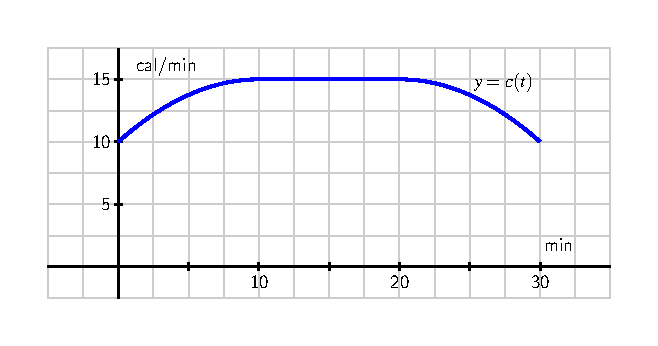
\includegraphics{figures/4_4_Act3.eps}
\caption{The rate $c(t)$ at which a person exercising burns calories, measured in calories per minute.} \label{F:4.4.Act3}
\end{center}
\end{figure}
\ba
	\item What is the exact total number of calories the person burns during the first 10 minutes of her workout?
	\item Let $C(t)$ be an antiderivative of $c(t)$.  What is the meaning of $C(30) - C(0)$ in the context of the person exercising?  Include units on your answer.
	\item Determine the exact average rate at which the person burned calories during the 30-minute workout.
	\item At what time(s), if any, is the instantaneous rate at which the person is burning calories equal to the average rate at which she burns calories, on the time interval $0 \le t \le 30$?
\ea
\end{activity}
\begin{smallhint}
\ba
	\item What are the units on the area of a rectangle found in a Riemann sum for the function $y= c(t)$?
	\item Use the FTC.
	\item Recall the formula for $c_{\mbox{\tiny{AVG}}[0,30]}$.
	\item Think carefully about which function tells you the instantaneous rate at which calories are burned.
\ea
\end{smallhint}
\begin{bighint}
\ba
	\item What are the units on the area of a rectangle found in a Riemann sum for the function $y= c(t)$?  What will be the units on area bounded by the curve?
	\item Use a definite integral and the FTC, as well as your work in (a).
	\item Recall the formula for $c_{\mbox{\tiny{AVG}}[0,30]}$.  Think about the relevant integral in terms of three subintervals: $[0,10]$, $[10,20]$, and $[20,30]$.
	\item Think carefully about which function tells you the instantaneous rate at which calories are burned, and consider your result in (c).
\ea
\end{bighint}
\begin{activitySolution}
\ba
	\item Since the units on a rectangle in a Riemann sum are cal/min for the height and min for the width, the units on the area of such a rectangle are calories, and hence the units on area under the curve $y = c(t)$ are given in total calories.  Hence, the total calories burned during the first 10 minutes of the workout is given by the definite integral $\int_0^{10} c(t) \, dt$.  We use the FTC and evaluate the integral, finding that
	\begin{eqnarray*}
		\int_0^{10} (-0.05t^2 + t + 10) \, dt & = & \left. \left( -\frac{0.05}{3} t^3 + \frac{1}{2} t^2 + 10t \right) \right|_0^{10} \\
				& = &  \left( -\frac{0.05}{3} (10)^3 + \frac{1}{2} (10)^2 + 10(10) \right) - (-0 + 0 + 0) \\
				& = & \frac{400}{3} \ \mbox{calories}.
	\end{eqnarray*}
	Thus, the person burned approximately 133.33 calories in the first 10 minutes of the workout.
	\item We observe first that by the Total Change Theorem, $C(30) - C(0) = \int_0^{30} C'(t) \, dt = \int_0^{30} c(t) \, dt$, and therefore, as discussed in (a), the meaning of this value is the total calories burned on $[0,30]$.
	\item The exact average rate at which the person burned calories on $0 \le t \le 30$ is given by 
	$$c_{\mbox{\tiny{AVG}}[0,30]} = \frac{1}{30-0} \int_0^{30} c(t) \, dt.$$
	To calculate $\int_0^{30} c(t) \, dt,$ we recognize that $c(t)$ is defined in piecewise fashion, and use the additive property of the definite integral, which tells us that 
	$$\int_0^{30} c(t) \, dt = \int_0^{10} c(t) \, dt +  \int_{10}^{20} c(t) \, dt +  \int_{20}^{30} c(t) \, dt.$$
	We know from our work in (a) that $\int_0^{10} c(t) \, dt = \frac{400}{3}$.  Since $c(t) = 15$ is constant on $10 \le t \le 20$, it follows that $ \int_{10}^{20} c(t) \, dt  = 15 \cdot 10 = 150$.  And finally, it is straightforward to show using $c(t) = -0.05t^2 + 2t - 5$ on $20 \le t \le 30$ that $\int_{20}^{30} c(t) \, dt = \frac{400}{3}$.  Hence,
	\begin{eqnarray*}
	\int_0^{30} c(t) \, dt & = & \int_0^{10} c(t) \, dt +  \int_{10}^{20} c(t) \, dt +  \int_{20}^{30} c(t) \, dt \\
			& = & \frac{400}{3} + 150 + \frac{400}{3} \\
			& = & \frac{1250}{3} \approx 416.67 \ \mbox{calories}.
	\end{eqnarray*}
	Now, it follows that the exact average rate at which calories were burned on $[0,30]$ is
	$$c_{\mbox{\tiny{AVG}}[0,30]} = \frac{1}{30-0} \int_0^{30} c(t) \, dt = \frac{1}{30} \cdot \frac{1250}{3} = \frac{1250}{90} \approx 13.89 \ \mbox{cal/min}.$$
	\item It makes sense intuitively that there must be at least one time at which the instantaneous rate at which calories are burned equals the average rate at which calories are burned, as it would be impossible for a continuous instantaneous rate of change to always be above its average value.  Since we know from (c) that $c_{\mbox{\tiny{AVG}}[0,30]} = \frac{125}{9}$, and $c(t)$ tells us the instantaneous rate at which calories are burned, it follows that we want to solve the equation
	$$c(t) = \frac{125}{9}.$$
From the graph, it appears that there are two such values of $t$ for which this equation is true, one in the first ten minutes, and one in the last ten.  For instance, solving
$$-0.05t^2 + t + 10 = \frac{125}{9},$$
it follows that $t = 10 \pm 10\sqrt{2}/3 \approx 14.714, 5.286$, only the second of which lies in $0 \le t \le 10$.  So one time at which the instantaneous rate at which calories are burned equals the average rate on $[0,30]$ is $t = 10 - 10\sqrt{2}/3 \approx 5.286.$  Similar reasoning shows that the other time is $t = 20 + 10\sqrt{2}/3 \approx 24.714$.
\ea
\end{activitySolution}
\aftera





